
\subsection{Zeichenfläche}

\subsubsection{Aufgaben}
Die Software soll dem Anwender ermöglichen in einer Zeichenfläche eine einfache Zeichnung zu erstellen. Dazu stehen im einige Werkzeuge zum Zeichnen von Quadraten, Kreisen und Linien zur Verfügung. Es soll jedoch auch möglich sein freihändig zu zeichnen, wodurch der Benutzer frei nach seinen Wünschen ein Bild malen kann. Die fertige Zeichnung soll anschließend automatisch in Befehle für den Roboter übersetzt werden, welcher die Figur nachzeichnet.

\subsubsection{Aufbau}
Für diese Aufgabe wird ein eigenes Control, das \textit{DrawingCanvas}, basierend auf dem \textit{InkCanvas} von WPF, sowie Teile der Edubot-API verwendet. Das \textit{InkCanvas} ermöglicht dem Benutzer das Erstellen von Freihandzeichnungen und kann sogar bestimmte Gestiken erkennen. Da diese Funktion in unserer Applikation jedoch nicht benötigt wird, haben wir uns nicht näher damit beschäftigt. Welche Aktion nun ausgeführt wird, wenn der Benutzer in das \textit{InkCanvas} klickt, hängt von der Eigenschaft \textit{InkCanvasEditingMode} ab, welche folgende Werte annehmen kann:
\begin{itemize}
\item EraseByPoint - Ermöglicht das Löschen einzelner Punkte
\item EraseByStroke - Ermöglicht das Löschen einzelner Pinselstriche, welche im weiteren Kontext auch \textit{Strokes}, genannt werden. Ein Pinselstrich sind alle Punkte die ein Benutzer in einem Durchzug zeichnet.
\item GestureOnly - Ermöglicht das Erkennen von Gestiken
\item Ink - Ermöglicht das Erstellen von Freihandzeichnungen
\item InkAndGesture - Ermöglicht das Erstellen von Freihandzeichnungen und das Erkennen von Gestiken.
\item None - Es wird keine Aktion ausgeführt
\item Select - Ermöglicht das Selektieren und Löschen von Pinselstrichen
\end{itemize}
In der Anwendung kommen die Modi \textit{EraseByPoint}, \textit{EraseByStroke}, \textit{Ink} und \textit{Select} zum Einsatz. Die Selektion letzterer erfolgt über eine, links vom \textit{InkCanvas} befindliche, Werkzeugleiste. Um dem Benutzer das Zeichnen von Kreisen, Rechtecken und Linien zu ermöglichen wird eine eigene Enumeration mit Namen \textit{InkCanvasDrawingMode} verwendet. Diese beinhaltet folgende Werte:
\begin{itemize}
\item Line - Ermöglicht das Erstellen von Linie
\item Rectangle - Ermöglicht das Erstellen von Rechtecken
\item Ellipse - Ermöglicht das Erstellen von Ellipsen
\item None - Es wird keine geometrische Form gezeichnet
\end{itemize}
Der vordefinierte \textit{InkCanvasEditingMode} \textit{None} kommt hierbei auch indirekt zum Einsatz, da er indiziert ob der Benutzer gerade eine der oben erwähnten geometrischen Figuren zeichnet. 
Da die Zeichenfläche zur schnelleren Verwendung auch die Undo/Redo-Funktion unterstützen sollte, wurde in unserem Control das Memento-Pattern verwendet. Außerdem soll die Zeichenfläche das Einzeichnen von, durch den aktuell verwendeten Adapter, nicht erreichbaren Punkten verhindern. Um den Arbeitsbereich auch visuell darzustellen umrandet das \textit{DrawingCanvas} den gültigen Bereich mit einer grauen Linie.

\subsubsection{Bedienung der Oberfläche}

\begin{figure}[H]
  \centering
  \begin{minipage}[t]{12 cm}
  	\centering
  	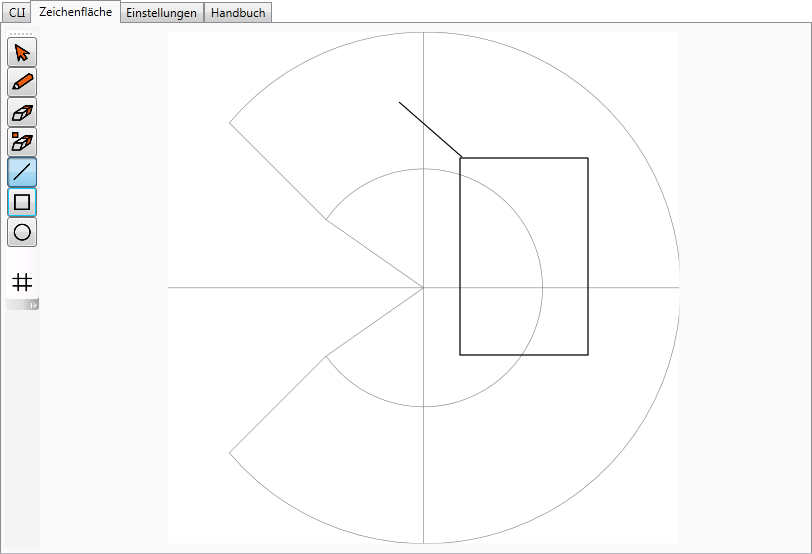
\includegraphics[width=12cm]{images/DrawingArea} 
    \caption{Die Zeichenfläche}
  \end{minipage}
\end{figure}

Um die Zeichenfläche zu nutzen, kann der Benutzer im linken Bereich des Tabs ein entsprechendes Werkzeug durch einen Klick auswählen. Anschließend kann er, wie aus anderen Zeichenanwendungen bekannt, die gewünschten Linien, Punkte und Formen einzeichnen. Die einzelnen Werkzeuge werden im folgenden erläutert:
\begin{itemize}
\item \textbf{Auswahl}: Wenn dieses Werkzeug ausgewählt wird, können Strokes (siehe Umsetzung für nähere Erklärung) ausgewählt und verschoben beziehungsweise über die Entfernen-Taste gelöscht werden.
\item \textbf{Freihand}: Wenn dieses Werkzeug ausgewählt wird, kann innerhalb der Zeichenfläche freihändig gezeichnet werden
\item \textbf{Radiergummi}: Wenn dieses Werkzeug ausgewählt wird, können beliebige Ausschnitte der Zeichnung gelöscht werden
\item \textbf{Stroke-Radiergummi}: Wenn dieses Werkzeug ausgewählt wird, können ganze Strokes mit einem Mausklick gelöscht werden
\item \textbf{Lineal}: Wenn dieses Werkzeug ausgewählt wird, können mittels "'Drag and Drop"' Linien in der Zeichenfläche gezeichnet werden
\item \textbf{Rechteck}: Wenn dieses Werkzeug ausgewählt wird, kann mittels "'Drag and Drop"' ein Rechteck gezeichnet werden
\item \textbf{Ellipse}: Wenn dieses Werkzeug ausgewählt wird, kann mittels "Drag and Drop" eine Ellipse gezeichnet werden
\end{itemize}

\subsubsection{Umsetzung der Zeichenfunktion}

DrawingCanvas
Wie im Aufbau erwähnt, wird dazu das, von \textit{InkCanvas} abgeleitete, \textit{DrawingCanvas}-Control verwendet. Im Konstruktor der Klasse werden zunächst die Methoden \textit{SetOrigin}, \textit{UpdateShape} und \textit{AddStrokes} an verschiedene Mausbewegungen gebunden und der \textit{EditingMode} auf \textit{InkCanvasEditingMode.Select} gesetzt. Weiters wurde das Property \textit{IsDrawingShape} definiert, welches angibt ob der Benutzer gerade eine geometrische Form zeichnet. Dazu wird lediglich geprüft ob der \textit{EditingMode} auf \textit{InkCanvasEditingMode.None} gesetzt ist und entsprechend ein Wert vom Typ Boolean zurückgeliefert. Weiters besitzt das \textit{DrawingCanvas} ein Property \textit{DrawingMode} vom Typ \textit{InkCanvasDrawingMode}, welches definiert welche geometrische Form der Benutzer gerade zeichnet.
\begin{itemize}
\item \textbf{SetOrigin}\\
Die Methode \textit{SetOrigin} wird aufgerufen, wenn der Benutzer die linke Maustaste drückt während sich der Mauszeiger im \textit{DrawingCanvas} befindet. Da Methode nur benötigt wird, um geometrische Formen zu zeichnen wird zuerst das \textit{IsDrawingShape}-Property überprüft. Liefert letzteres true zurück, so wird der aktuelle Punkt in der globalen Variable origin vom Typ \textit{Point} gespeichert.
\item \textbf{UpdateShape}\\
Die Methode \textit{UpdateShape} wird aufgerufen, wenn der Benutzer den Mauszeiger innerhalb des Controls bewegt. Auch hier wird zuerst das \textit{IsDrawingShape}-Property überprüft. Ist dieses auf true gesetzt, so wird die \textit{InvalidateVisual}-Methode aufgerufen, welche das \textit{DrawingCanvas} neu zeichnet. Dazu ruft WPF die \textit{OnRender}-Methode der Klasse auf, in welcher geprüft wird ob gerade eine geometrische Form gezeichnet wird und um welche es sich handelt. Abhängig von diesen Faktoren wird mit Hilfe eines \textit{DrawingContext}-Objekt die entsprechende Form gezeichnet.
\item \textbf{AddStrokes}\\
Die Methode \textit{AddStrokes} wird aufgerufen, wenn der Benutzer die linke Maustaste loslässt. Zuerst wird erneut das \textit{IsDrawingShape}-Property geprüft und anschließend die aktuelle Position des Mauszeigers gespeichert. Da wir nun über den Ausgangspunkt, repräsentiert durch die origin-Variable, als auch den Endpunkt \textit{currentPoint} verfügen, ist die Größe der geometrischen Form definiert.
Mit Hilfe einer \textit{switch}-Kontrollstruktur wird nun ermittelt, welche Form der Benutzer gezeichnet hat und ein entsprechendes \textit{Stroke}-Objekt erzeugt. Ein \textit{Stroke} enthält eine Menge an Punkten, die sogenannten \textit{StylusPoints}, welche, wenn das Objekt zur \textit{Stroke}-Collection der \textit{InkCanvas}-Klasse hinzugefügt wird, gezeichnet werden. Zwischen den angegebenen Punkten wird jeweils eine Linie gezeichnet, wodurch ein \textit{Stroke}-Objekt mit entsprechend definierten Punkten eine geometrische Form darstellen kann.
\end{itemize}

\textbf{Umrechnung der geometrischen Formen in Strokes}
Wie oben erwähnt, findet in der \textit{AddStrokes} Methode die Umrechnung der, vom Anwender gezeichneten Form, in entsprechende Strokes statt. 
\begin{itemize}
\item \textbf{Line}\\ 
\begin{lstlisting}[language = CSharp, captionpos=b, caption={Linie in Strokes konvertieren}]
StylusPointCollection line = new StylusPointCollection();
line.Add(new StylusPoint(origin.X, origin.Y));
line.Add(new StylusPoint(currentPosition.X, currentPosition.Y));
stroke = new Stroke(line);
Strokes.Add(stroke);
OnStrokeCollected(new InkCanvasStrokeCollectedEventArgs(stroke));
\end{lstlisting}
Hierbei wird ein \textit{Stroke}-Objekt mit zwei \textit{StylusPoints}, dem Ursprungs- und dem Endpunkt, generiert.
\item \textbf{Rectangle}\\ 
\begin{lstlisting}[language = CSharp, captionpos=b, caption={Rechteck in Strokes konvertieren}]
StylusPointCollection rect = new StylusPointCollection();
rect.Add(new StylusPoint(origin.X, origin.Y));
rect.Add(new StylusPoint(currentPosition.X, origin.Y));
rect.Add(new StylusPoint(currentPosition.X, currentPosition.Y));
rect.Add(new StylusPoint(origin.X, currentPosition.Y));
rect.Add(new StylusPoint(origin.X, origin.Y));
if (rect.Count > 0)
{
	stroke = new Stroke(rect);
	Strokes.Add(stroke);
	OnStrokeCollected(new InkCanvasStrokeCollectedEventArgs(stroke));
}
\end{lstlisting}
Hierbei wird ein \textit{Stroke}-Objekt mit fünf \textit{StylusPoints} generiert. 
\begin{align}
P_1 = (x_{origin} / y_{origin})\\
P_2 = (x_{currentPoint} / y_{origin})\\
P_3 = (x_{currentPoint} / y_{currentPoint})\\
P_4 = (x_{origin} / y_{currentPoint})\\
P_5 = (x_{origin} / y_{origin})
\end{align}

\item \textbf{Ellipse}\\ 
\begin{lstlisting}[language = CSharp, captionpos=b, caption={Ellipse in Strokes konvertieren}]
StylusPointCollection ellipse = new StylusPointCollection();
int radiusX = (int)(currentPosition.X - origin.X) / 2;
int radiusY = (int)(currentPosition.Y - origin.Y) / 2;
int segmentCount = (int)(Math.Sqrt(radiusX * radiusX + radiusY * radiusY)*4);
double dTheta = 2 * Math.PI / segmentCount;
double theta = 0;
Point center = new Point(origin.X + radiusX, origin.Y + radiusY);                        
 int currentX = (int) center.X + radiusX;
int currentY = (int) center.Y;
for (int segment = 0; segment < segmentCount; segment++)
{
	theta += dTheta;
           currentX = (int) (center.X + radiusX * Math.Cos(theta));
           currentY = (int) (center.Y + radiusY * Math.Sin(theta));
           ellipse.Add(new StylusPoint(currentX, currentY));
}
if (ellipse.Count > 0)
{
	stroke = new Stroke(ellipse);
          Strokes.Add(stroke);
          OnStrokeCollected(new InkCanvasStrokeCollectedEventArgs(stroke));
 }
\end{lstlisting}
Hierbei wird ein \textit{Stroke}-Objekt mit einer, von der Ellipsengröße abhängigen, Menge an \textit{StylusPoints} generiert. Zur Berechnung der Ellipsenpunkte kommt ein ähnliches Verfahren wie bei zirkularen Interpolation zum Einsatz.
\begin{enumerate}
\item Radien der Ellipse berechnen\\
Zuerst müssen die zwei Radien der Ellipse $r_x$ und $r_y$ mit Hilfe des Ursprungs- und des Endpunkts berechnet werden.
\begin{align}
r_x &= x_{origin} - x_{currentPoint}\\
r_y &= y_{origin} - y_{currentPoint}
\end{align}
\item Anzahl der Ellipsensegmente ermitteln\\
Anschließend wird die ungefähre Anzahl der zu berechnenden Außenpunkte mit folgender Formel berechnet.
\begin{align}
n = 4 \sqrt{r_x^2+r_y^2}
\end{align}
\item Winkelsteigung berechnen\\
Im nächsten Schritt wird die Steigung des Winkels pro berechnetem Punkt kalkuliert.
Anmerkung: Da die \textit{Math.Sin} beziehungsweise \textit{Math.Cos}-Methode nur einen Winkel in Radiant übernimmt, wird hier in der Anwendung $\frac{2\pi}{n}$ gerechnet.
\begin{align}
k_{\theta} = \frac{360^\circ}{n}
\end{align}
\item Mittelpunkt berechnen\\
Nun wird der Mittelpunkt, erneut mit Hilfe des Ursprungs- und Endpunkts, berechnet.
\begin{align}
m_x &= x_{origin} + r_x\\
m_y &= y_{origin} + r_y
\end{align}
\item Berechnung der Außenpunkte\\
Zuerst wird ein Startpunkt für die weitere Berechnung festgelegt, welcher wie folgt definiert ist:
\begin{align}
s_x &= m_x + r_x\\
s_y &= m_y
\end{align}
Anschließend werden in einer Schleife die Zwischenpunkte berechnet und als als \textit{StylusPoints} zum \textit{Stroke} hinzugefügt. Der $i$-te Zwischenpunkt, definiert durch $p_x$ und $p_y$, wird nach folgender Formel berechnet:
\begin{align}
p_x &= m_x + r_x \cos(ik_\theta)\\
p_y &= m_y + r_y \sin(ik_\theta)
\end{align}
\end{enumerate}

\item
\end{itemize}
Vor dem Hinzufügen des \textit{Strokes} wird geprüft ob er \textit{StylusPoints} enthält, da es in Ausnahmefällen dazu kommen kann das keine Punkte berechnet wurden. Ein Beispiel für einen solchen Ausnahmefall wäre eine Ellipse mit Radius 0, welche durch einen versehentlichen Klick in die Zeichenfläche berechnet wird. Enthält der \textit{Stroke} jedoch Punkte, so wird er über das \textit{OnStrokeCollected}-Events, verpackt in einem \textit{StrokeCollectedEventArgs}-Objekt, der \textit{Stroke}-Collection des \textit{InkCanvas} hinzugefügt. 

\subsubsection{Umsetzung der Befehlsgenerierung}

Die zu einem Zeitpunkt im \textit{DrawingCanvas} enthaltenen Strokes können mit Hilfe der \textit{GenerateMovementCommands}-Methode in eine Liste aus \textit{ICommand}-Objekten umgeformt werden. Dazu wird durch die vorhandenen \textit{Strokes} und wiederum deren \textit{StylusPoints} iteriert und je ein \textit{MVSCommand} mit dem nächsten \textit{StylusPoint} als Zielpunkt erstellt. 
Die Befehle werden dabei in derselben Reihenfolge erzeugt wie die \textit{Strokes} gezeichnet wurden. Weiters wird zwischen zwei Punkten geprüft ob die Achskonfiguration zum Erreichen dieses Punkts geändert werden muss.
Dazu bedient sich das \textit{DrawingCanvas} der Methoden der \textit{Kinematics}-Klasse.
Für Strecken zwischen zwei \textit{Strokes} wird das Werkzeug ausgeschaltet und nur zwischen ersten und letztem \textit{StylusPoint} des \textit{Strokes} wieder eingeschaltet.


\subsubsection{Umsetzung der Undo/Redo-Funktion}
Um Aktionen innerhalb der Zeichenfläche rückgängig beziehungsweise wiederholbar zu machen, wird das sogenannt Memento-Pattern verwendet. Letzteres ist eine Software-Architektur-Muster, welches von der "'Gang of Four"', einer Gruppe von Programmierern, für spezielle Aufgaben entwickelt wurde. Das Memento-Pattern eignet sich hervorragend für Aufgaben wie Undo/Redo-Operationen, weshalb es in der \textit{DrawingCanvas}-Klasse verwendet wird.\\
Die Idee dahinter ist, dass für jede Operation ein sogenanntes Memento erzeugt und einer chronologisch geordneten Liste hinzugefügt wird. Das Memento enthält genauere Informationen über die ausgeführte Operation. Durch Iteration der Liste können alle von Beginn an durchgeführten Operationen nachvollzogen werden.\\
\begin{lstlisting}[language = CSharp, captionpos=b, caption={Die Memento-Klasse}]
class Memento{
            string operation;

            public string Operation
            {
                get { return operation; }
                set { operation = value; }
            }

            StrokeCollection strokes;

            public StrokeCollection Strokes
            {
                get { return strokes; }
                set { strokes = value; }
            }
        }
\end{lstlisting}
Im Falle des DrawingCanvas enthält ein Memento folgende Properties:
\begin{itemize}
\item Operation\\
Das \textit{Operation}-Property ist vom Typ String und definiert ob ein \textit{Stroke} hinzugefügt oder gelöscht wurde. Dabei steht "add" für Hinzufügen und "del" für Löschen.
\item Stroke\\
Das \textit{Stroke}-Property beinhaltet den, von der Operation betroffenen, \textit{Stroke}. Dadurch kann das entsprechende Objekt einfach aus der \textit{Stroke}-Collection des \textit{InkCanvas} entfernt beziehungsweise hinzugefügt werden.
\end{itemize}

Die \textit{Memento}s werden in zwei Stacks, dem \textit{undoBuffer} und dem \textit{redoBuffer}, verwaltet. Ein Stack, auch Kellerspeicher genannt, stapelt mit Hilfe der \textit{Push}-Methode hinzugefügte Elemente übereinander beziehungsweise gibt bei Aufruf der \textit{Pop}-Methode das zuletzt hinzugefügte Element zurück und entfernt dieses aus dem Stapel.\\
Um ein \textit{Memento} hinzuzufügen wurde die Methode \textit{AddMemento} im \textit{DrawingCanvas} implementiert und im Konstruktor der Klasse dem \textit{StrokeCollected}- beziehungsweise \textit{StrokeErased}-Event zugewiesen. Diese Events werden beim Zeichnen und Löschen von Pinselstrichen oder Punkten ausgelöst. Die Klasse merkt sich die durchgeführte Operation durch ein neues Memento und kann diese bei Bedarf rückgängig machen, wozu lediglich eine entsprechende Gegenoperation durchgeführt wird.
\begin{itemize}
\item \textbf{AddMemento}\\
Die Methode \textit{AddMemento} übernimmt als Parameter ein object \textit{sender}, welches das Objekt enthält, dass das Ereignis verursacht hat, sowie ein Objekt vom Typ \textit{EventArgs} mit näheren Details zum Ereignis. Bei Aufruf dieser Methode wird zuerst die globale Variable \textit{addMemento} geprüft, welche angibt ob ein \textit{Memento} für diese Operation hinzugefügt werden soll. Der nähere Zweck dieser Variable wird in der \textit{Undo} beziehungsweise \textit{Redo}-Methode beschrieben. Ist \textit{addMemento} auf true gesetzt, so wird geprüft um welche spezifische Klasse es sich beim \textit{EventArgs}-Objekt handelt.\\
Handelt es sich dabei um ein \textit{InkCanvasStrokeCollectedEventArgs}-Objekt so indiziert dies, das ein neuer \textit{Stroke} hinzugefügt wurde. Anschließend wird ein \textit{Memento} mit der \textit{Operation} "add" und dem, in den Event-Argumenten enthaltenen, \textit{Stroke} erzeugt und in den \textit{redoBuffer} gegeben. Sollte es sich beim \textit{EventArgs}-Objekt um ein \textit{InkCanvasStrokeEraseEventArgs}-Objekt handeln, so wird im erstellten \textit{Memento} "del" als \textit{Operation} angegeben. Zuletzt wird noch der \textit{redoBuffer} geleert, da der Benutzer eine neue Aktion durchgeführt und deshalb die \textit{Memento}s über zuvor rückgängig gemachte Aktionen verworfen werden müssen.
\item \textbf{Undo}\\
Die Methode \textit{Undo} überprüft zuerst ob sich Elemente im \textit{undoBuffer} befinden. Sollte dies der Fall sein, so wird das oberste \textit{Memento} im Stapel entfernt und das \textit{Operation}-Property überprüft. Wenn "add" als Operation angegeben wurde, so muss der entsprechende \textit{Stroke} gelöscht werden, um die Aktion rückgängig zu machen. Dazu wird die \textit{Remove}-Methode der \textit{Strokes}-Collection mit dem, im \textit{Memento} gespeicherten, \textit{Stroke} aufgerufen. Handelt es sich bei der \textit{Operation} um "del", so wird der betroffene \textit{Stroke} mit Hilfe der \textit{Add}-Methode der \textit{Strokes}-Collection wieder hinzugefügt. Zuletzt wird die soeben rückgängig gemachte Aktion zu unserem \textit{redoBuffer} hinzugefügt, um sie bei Bedarf wiederholen zu können.\\
Das manuelle Bearbeiten der \textit{Strokes}-Collection führt erneut zu \textit{StrokesCollected} beziehungsweise \textit{StrokesErased}-Events, weshalb auch unsere \textit{AddMemento}-Methode aufgerufen wird. Da wir in diesem Fall jedoch nicht erneut ein \textit{Memento} erzeugen wollen, setzen wir vor Hinzufügen und Löschen von \textit{Strokes} die \textit{addMemento}-Variable auf false. Erst nach Abschluss aller Aktionen in der \textit{Undo}-Methode wird diese Variable wieder auf true gesetzt und neue \textit{Memento}s erzeugt. 
\item \textbf{Redo}\\
Die Methode \textit{Redo} überprüft zuerst ob sich Elemente im \textit{redoBuffer} befinden. Anschließend wird das oberste \textit{Memento} aus dem Stapel geholt und die, im \textit{Operation}-Property gespeicherte, Aktion ausgeführt. Hierbei kommen dieselben Methoden wie in der \textit{Undo}-Methode zum Einsatz, nur das hierbei die im \textit{Memento} angegebene Operation und nicht die Gegenoperation durchgeführt wird. Weiters wird auch hier während Ausführung der Methode die \textit{addMemento}-Variable auf false gesetzt.
\end{itemize}

